\section{Data}


Data presented is at the county level with the exception of planting and silking date data for Iowa. The county level yield data is given by annual observations of the average yield in each county, while the weather variables are calculated based on daily observations of temperature and precipitation.

\subsection{Ontario}

Yield data for Ontario was obtained from the Ontario Ministry of Agriculture, Food and Rural Affairs (OMAFRA). This data includes annual county level average yield observations from 1950 to 2013. Weather data is from Environment Canada weather station records. The county level observations were determined by taking a distance weighted average of daily weather variable observations with respect to county centroids. The daily weather observations include maximum and minimum temperatures, as well as daily precipitation totals. 

\subsection{Iowa}

County level yield data for Iowa from 1955-2012 was collected from the National Agricultural Statistics Service (NASS). The weather data was generated by the National Oceanic and Atmospheric Adminstration (NOAA), and contains daily maximum and minimum temperatures, as well as daily precipitation totals for each county. A data set containing information on planting and silking dates by year in Iowa was also used. This data set was at the agricultural district level for the years 1974-2012, where each district contains about 10 counties. Each year of data for a given agricultural district gives the percentages of total acreage planted by given dates. This data was also obtained from the NASS. 



\section{Conceptual Corn Yield Model}

The conceptual model represents corn yield as a function of both weather and non-weather  variables, and time. Agricultural technology has changed yield distributions in both areas considered in this study as discussed in the introduction; this implies that the yield model must depend on time. Given that the relationship between yield and precipitation may have changed over the study period, a time variant function representing the effect of precipitation on yield was included. Thus the conceptual model is represented by the equation below.

\begin{equation}
Y=f(T,h(PCP,T),X,M)
\end{equation}

$Y$ represents yield, $T$ represents time, $PCP$ represents precipitation $X$ represents all other weather variables impacting yield, and $M$ represents any non-weather variables which affect yield. $h$ is a function of time and precipitation which represents the time-variant effect of precipitation level on yield and $f$ is a function which determines yield level based on these inputs. 

\section{Empirical Model}


A linear functional form was used for the yield function $f$. The effect of precipitation on yield was allowed to vary depending on the amount of precipitation received. This was done to capture the fact that precipitation is a positive yield determinant but can be detrimental in excess \citep{rosenzweig2002increased}. To empirically model this relationship, a piecewise continuous linear function with two threshold points (break points) was used. Each of the thresholds mark points of slope change. Below the lower threshold, $\pi_l$, precipitation is assumed to have a strong positive effect on yields. When precipitation levels are between the two thresholds the effect should continue to be positive but the slope should be less steep. Finally, when precipitation levels exceed the second threshold, $\pi_u$, the slope should become negative to represent the expected yield damaging effect of excessive precipitation. The space between these thresholds represents the ideal precipitation range, the interval at which the crop is receiving high enough levels of precipitation to attain high yields but not too much to become detrimental. The relationship is demonstrated visually in Figure 3.1.

\begin{figure}
 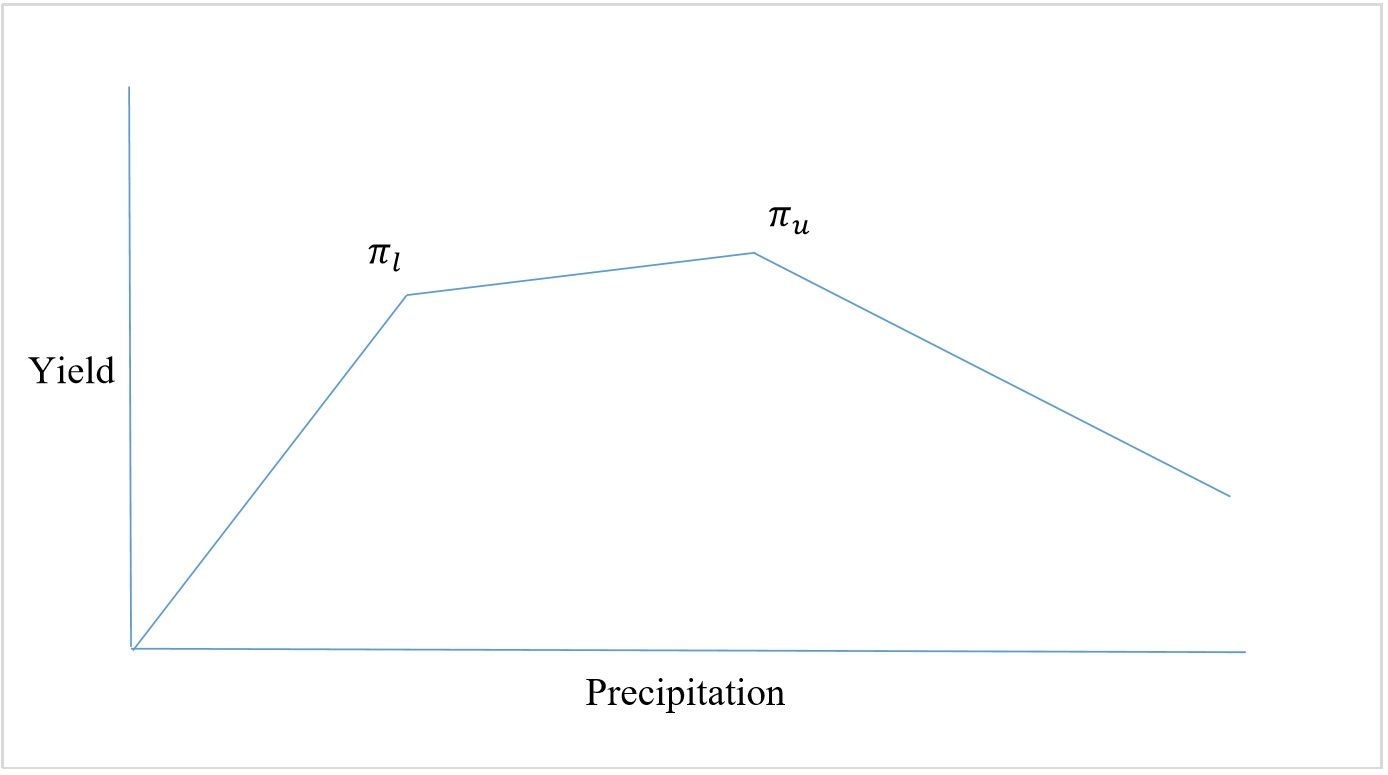
\includegraphics[width=\textwidth]{2threshold.jpg}
    \caption{Approximation of the yield precipitation relationship for use in empirical model}
 \end{figure}
    
In order to use this structure to consider the relationship between yield and precipitation, two additional precipitation variables which indicate when precipitation levels are above the lower and upper threshold values respectively, are included in the model. Precipitation demand is expected to have increased over time due to the increase in plants and yield per acre. Approximating the effect of precipitation on yields using a piecewise linear function as described above, this increased demand would be interpreted as increased lower and upper threshold levels. To allow for this in the empirical model, the threshold levels are allowed to change linearly through time.

\begin{equation}
\pi_l = a_l + b_lT
\end{equation}

\begin{equation}
\pi_u = a_u + b_uT
\end{equation}

Where $T$ represents time, $\pi_l$ is the lower threshold, $\pi_u$ is the upper threshold and $a_l,b_l,a_u,b_u$ are unknown parameters which determine the threshold levels at a given point in time. Finally, due to the large increases in expected yield during the period of study, a trend is included. In Iowa the yield over time appears to follow an approximately linear trend over the entire study period. In Ontario however it can be seen that yields began to rise more steeply beginning around year 2000.

    
\begin{figure}[!hb]
  \centering
  \begin{minipage}[b]{0.49\textwidth}
    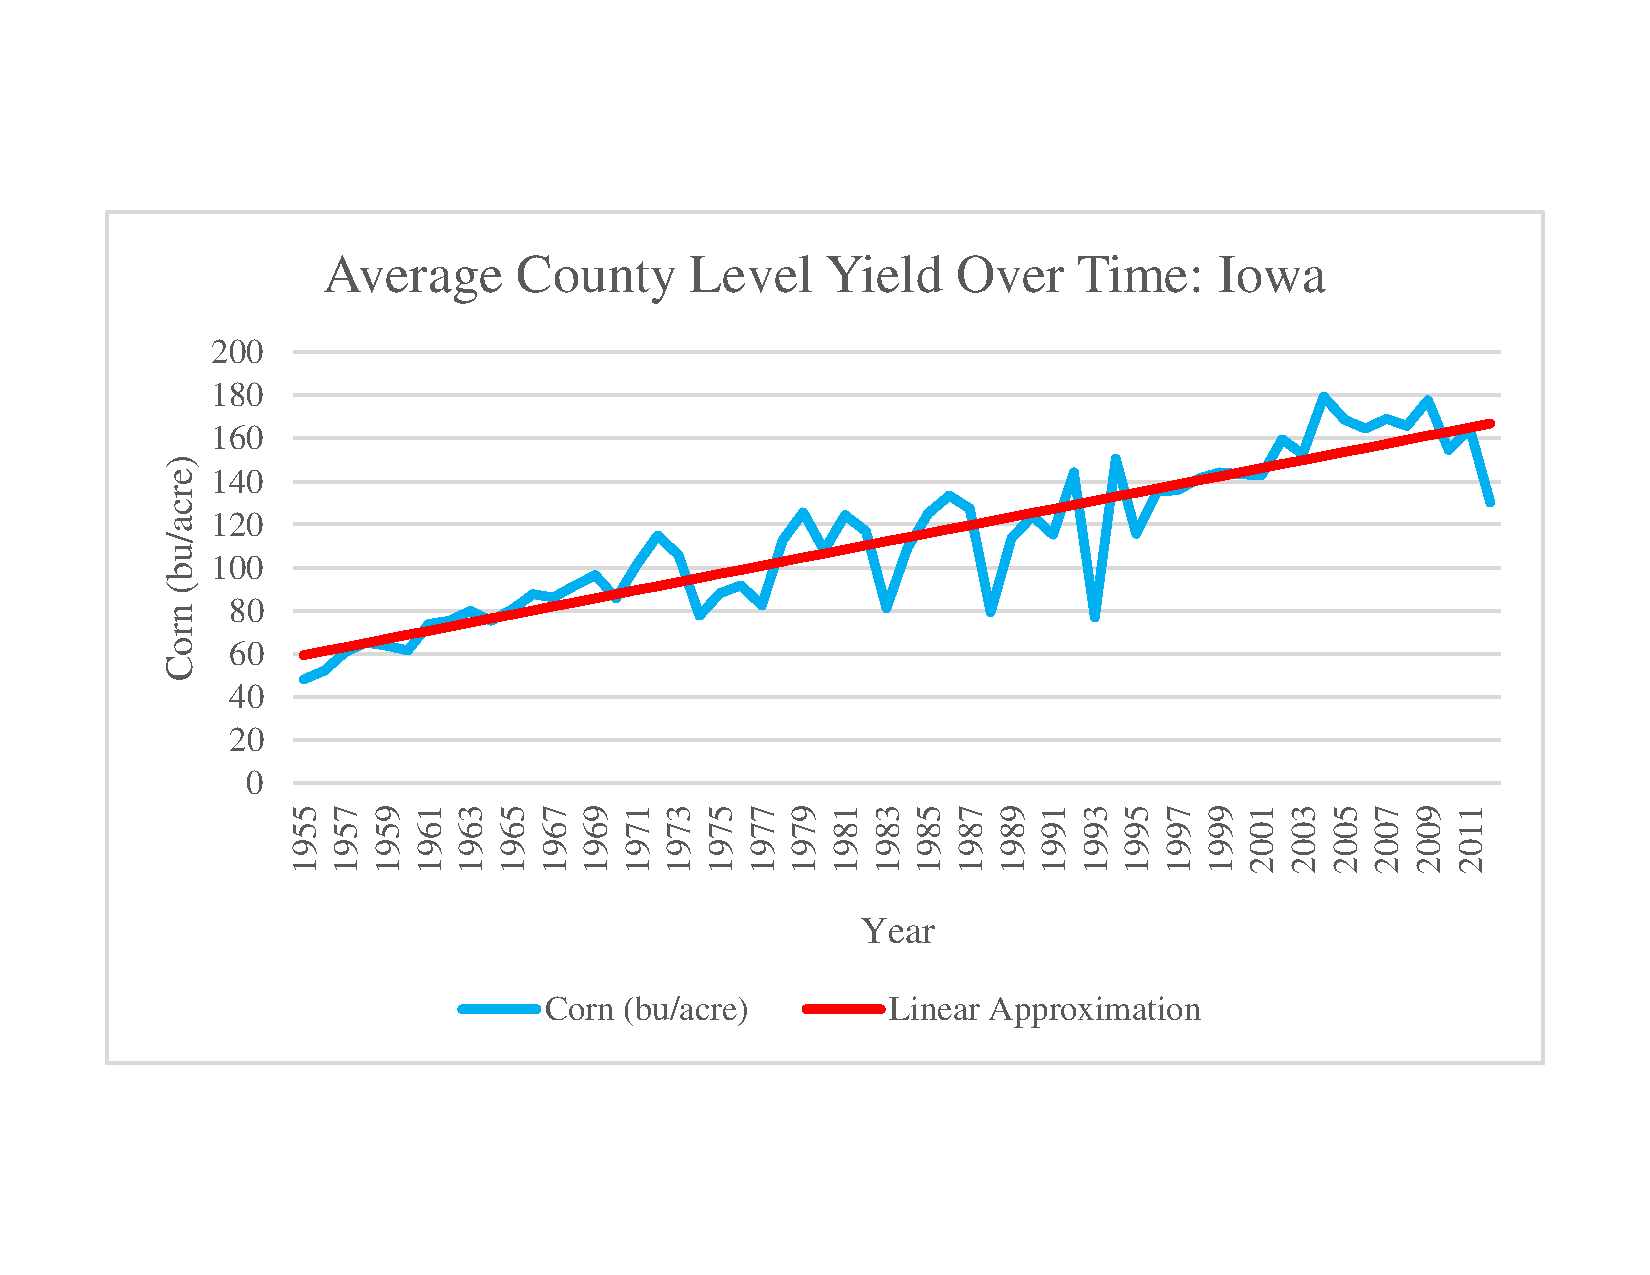
\includegraphics[width=\textwidth]{YieldIowa.pdf}
    \caption{Plot of Yield and Piece-wise Linear Approximation - Iowa}
  \end{minipage}
  \hfill
  \begin{minipage}[b]{0.49\textwidth}
    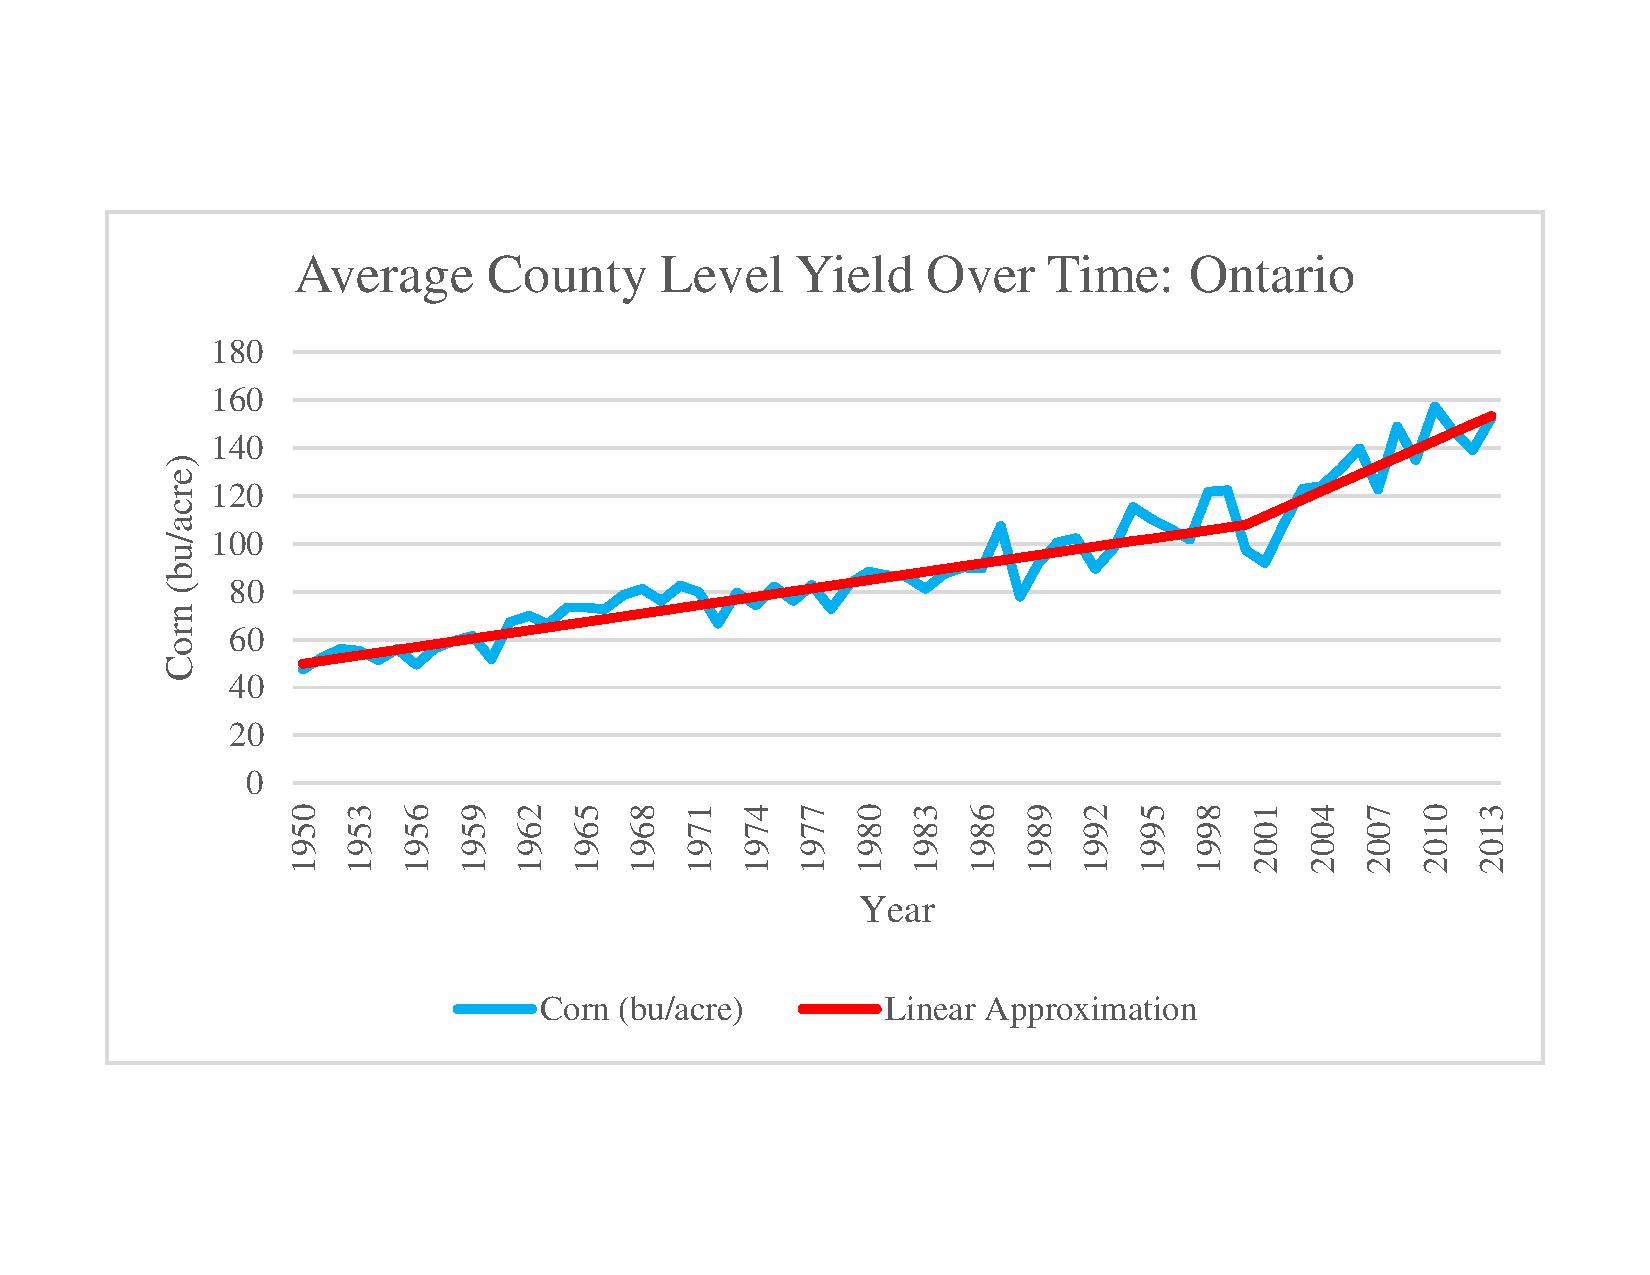
\includegraphics[width=\textwidth]{YieldOnt.pdf}
    \caption{Plot of Yield and Piece-wise Linear Approximation - Ontario}
  \end{minipage}
\end{figure}   
 
    
 Due to these observations, a single linear trend was included in the Iowa model, and a piecewise linear trend with a break point at 2000 in the Ontario model. This results in the following empirical models for Ontario and Iowa respectively:

\begin{equation}
Y=\beta_0+\beta_1p+\beta_2(max(PCP,\pi_u)-\pi_u)+\beta_3(max(PCP,\pi_h)-\pi_h)+\beta_4t+\beta_5(max(T,50)-50)+\delta X_{Ont}+\epsilon
\end{equation}

\begin{equation}
Y=\beta_0+\beta_1p+\beta_2(max(PCP,\pi_u)-\pi_u)+\beta_3(max(PCP,\pi_h)-\pi_h)+\beta_4t+\delta X_{Iowa}+\epsilon
\end{equation}

Where the $\beta$'s are scalar and unknown parameters, $\delta$ is a vector of unknown parameters, $t$ is the number of years since the beginning of the study period (1950 in Ontario and 1955 in Iowa), $X$ is a matrix of relevant weather variables in each location, and $\epsilon$ is an error term. The impact of omitted weather variables, as well as  of non-weather variables which affect yield, will be captured in the error term. A restriction on this model was also considered in which the upper and lower thresholds are equal to each other, thus collapsing to a single threshold model.

\section{Variable Choice}

An examination of the literature demonstrates that the choice of independent variables to include in the model is not trivial. Based on the results found in the literature review it appears that including a measure of vapour pressure deficit in addition to measures of precipitation and temperature can increase the fit of the model \citep{roberts2012agronomic}. Considering weather variables timed to growth stage has also been shown to increase the fit of the model as compared to averages over the growing season or monthly weather variables \citep{dixon1994estimating, ozkan2002impacts}. Schlenker and Roberts found that including the cumulative temperature over the growing season, by considering daily temperatures and modelling their distribution over each day, led to better results than using averages \citep{schlenker2009nonlinear}. A sin curve approximation of daily temperature distribution to calculate growing degree days will therefore be included. This variable is calculated using the method described in \cite{snyder1985hand}. 

Based on these results and on data availability, the following independent weather variables were considered for inclusion in the model:  accumulated and average precipitation, accumulated and average vapour pressure deficit, growing degree days, cold degree days, freezing degree days and extreme heat degree days. The timing of key growth stages was also considered so that the levels of the independent weather variables during each stage could be calculated. This was done due to account for changing relationships between yield and weather variables over the growing season. 

Precipitation is needed at a very low level in the initial growth stage. The crop water demand gradually increases throughout the vegetative stage as the plant progressively grows taller and develops more leaves \citep{OMAFRA}. Once all the leaves are developed the reproductive growth stages begin. Silks emerge from the corn plant and are receptive to pollination.  During this small period of time where pollen is being shed and silks have emerged the plant is very sensitive to environmental stress, such as drought or extreme heat \citep{OMAFRA}. The beginning of the silking and pollination stage is approximated by accumulated growing degree days (GDD) \cite{neild1987growing}. The GDD begin accumulating at the time of planting, and the various growth stages begin approximately after some particular GDD accumulation is reached. Unfortunately, a complete data set for planting days by county could not be found which made the determination of growth stage timing, and the subsequent creation of appropriate weather variables, difficult. The number of days to include within a particular growth stage is also somewhat unclear. For example, pollination takes about 7 days after the beginning of the silking period \citep{OMAFRA}, however, the exact amount of days will change from farm to farm. In order to increase the probability that the timed weather variables would capture the correct timing for most farms within the county, a few days were added on either end of the estimated beginning and end dates of the growth stage.

Given that the best method for timing growth stages is not clear, various timings and combinations of the variables were considered and tested in order to select the preferred set of independent variables for Iowa and Ontario respectively. On average silking and pollination occur at some point in July but the exact timing can vary based on environmental conditions.  Due to the difficulties involved in estimating the timing of growth stages, models with variables timed according to month were also considered. 

\section{Weather Data Timing}

As described above the weather variables were timed to particular stages of growth based on estimated planting dates and accumulated heat units. The heat units were measured using Growing Degree Days (GDD) in both Iowa and Ontario. The demand for precipitation is the relationship of interest and therefore the choice of how to time variables was especially focused on the agronomic yield-water relationship. As mentioned above precipitation has the most marked effect on yield when the corn plant is undergoing silking and pollination. Therefore estimation of the timing of the silking stage was the main focus.

In Iowa, access to a data set at the regional level identifying the percentage of corn acres which had been planted by each week between mid April and mid June was obtained. The data set also provided the percentage of acres where silking had begun by certain dates between early July and early August. Using this data set, the date at which 50 percent of corn acres had been planted in each region was calibrated. The resultant regional level 50th percentile date was then used as the planting date for each county within that region. The regional silking dates were calibrated in an analogous fashion. This data was available only for the years 1974-2012 with the exception of years 1987 and 1992, which only contained planting observations for 1 week in the season and were omitted. In order to estimate the planting and silking dates for the remaining years in the study, a linear model for planting dates was developed based on the planting and silking data described above. This model used weather in April as a predictor for planting date. Weather conditions in April were also used by \cite{gupta1985predicting} as an indicator of planting date. A trend was included in order to correct for the changes in farm management practices over time, which have generally led to earlier planting dates \citep{kucharik2006multidecadal}. The planting date model which was estimated was as follows:

\begin{equation}
  planting_{day}=\beta_0+\beta_1T+\beta_2Temp_{April}+\beta_3VPD_{April}+\beta_4PCP_{April}
\end{equation}

Where $Temp_{April}$ is the mean of the average daily temperature in April, $PCP_{April}$ and $VPD_{April}$ are averages of the daily precipitation and vapor pressure deficit totals in April, and $T$ represents time. This model was estimated using the calibrated county level planting dates for years 1974-2012 excluding 1987 and 1992.

The result of the planting date model estimation is shown below:



% Table created by stargazer v.5.2 by Marek Hlavac, Harvard University. E-mail: hlavac at fas.harvard.edu
% Date and time: Sun, Dec 11, 2016 - 8:42:16 PM
% Requires LaTeX packages: dcolumn 
\begin{table}[H] 
  \caption{Planting Date Model Results} 
  \label{} 
\begin{tabular}{@{\extracolsep{5pt}}lc} 
\\[-1.8ex]\hline 
\hline \\[-1.8ex] 
 & \multicolumn{1}{c}{\textit{Dependent variable:}} \\ 
\cline{2-2} 
\\[-1.8ex] & \multicolumn{1}{c}{planting\_day} \\ 
\hline \\[-1.8ex] 
 T & -0.310^{***} \\ 
  & (0.009) \\ 
 Temp$_{April}$ & -0.245^{**} \\ 
  & (0.098) \\ 
 VPD$_{April}$ & -12.567^{***} \\ 
  & (0.900) \\ 
 PCP$_{April}$ & 1.688^{***} \\ 
  & (0.084) \\ 
 Constant & 151.484^{***} \\ 
  & (0.664) \\ 
\hline \\[-1.8ex] 
Observations & \multicolumn{1}{c}{3,663} \\ 
R$^{2}$ & \multicolumn{1}{c}{0.485} \\ 
Adjusted R$^{2}$ & \multicolumn{1}{c}{0.484} \\ 
Residual Std. Error & \multicolumn{1}{c}{6.124 (df = 3658)} \\ 
F Statistic & \multicolumn{1}{c}{860.533$^{***}$ (df = 4; 3658)} \\ 
\hline 
\hline \\[-1.8ex] 
\textit{Note:}  & \multicolumn{1}{r}{$^{*}$p$<$0.1; $^{**}$p$<$0.05; $^{***}$p$<$0.01} \\ 
\end{tabular} 
\end{table} 

This model was used to predict planting date for the years in the study which were not included in the planting data set. For the years included in the planting data set, the calibrated planting and silking dates for each region were used for all the counties in that region. The planting dates resulting from this method were then used as  as the starting point for timing relevant growth stages.

 Planting data equivalent to that used for Iowa could not be accessed in Ontario. Given that there was no planting data, a planting date model could not be estimated. The method which has been favoured by OMAFRA for estimating planting date was used instead. This method assigns planting date to be the first day in the planting season where the previous 3 days have had average temperatures greater than or equal to 12.8 degrees Celsius \citep{OMAFRAhybrid}.

Since the warm weather variables HDD and GDD mostly attain positive values during the middle of the growing season (especially HDD) when they have the largest effect on the plant, seasonal totals of GDD and HDD were used to account for warm weather effects and the timing was not changed when testing the various models. Similarly, the cold weather variables are only likely to have non-zero values during the beginning and possibly end of the season, and were also not adjusted according to different timing methods.

Six different ways of timing variables were tested, and for each timing method 7 different combinations of the potential model variables were considered. Since Iowa and Ontario have slightly different climates and have different histories when it comes to corn production they were modelled separately. The different timings varied the amount of buffering added to the planting estimates, and also the number of subsets of growth stage that were considered. The details of the different timing options tested, and their agronomic significance, as well as the different combinations of variables considered are included in the  appendix in section 8.3.


\section{Estimation of Various Models for variable choice}

In order to select the variables which would be used in the model, several combinations of independent variables were considered. A linear yield model was estimated with each potential combination of independent variables and each timing method, and the resulting $R^2$ was stored. The choice of variables to include in the model for further analysis was determined based on the resulting adjusted $R^2$ from each model estimation, as well as on the interpretation of the model coefficients.

\subsection{Spatial Autocorrelation}

The model described in the empirical framework is a linear yield model based on weather variables and trend. In order to justify the estimation of this model using Ordinary Least Squares (OLS), the assumption that all of the observations are independent and identically distributed should hold at least approximately. Given the spatial nature of this data, the assumption of independence is hard to justify. Many unmeasured and unobserved variables such as soil moisture, soil temperature, seed hybrid, and choices relating to farm management affect yields. The effects of these excluded variables will be captured by the error term in the model. Some of these unobserved variables are determined by the local weather conditions which are certainly spatially correlated. Others relate to cultural norms and practices which are also likely to be correlated across space. This leads to the conclusion that the error terms in the model will most likely be spatially correlated. This is modelled as shown below, where X represents all variables included in the yield model including the constant term, trend and  precipitation effects:

\begin{equation}
y_{it}=X_{it}\delta+u_{it}
\end{equation}

\begin{equation}
u_{it}=\rho\sum_{j=1}^{n}(w_{ij}u_{jt})+\epsilon_{it}
\end{equation}

 The $i$ and $j$ subscripts are county indicators, while the $t$ subscript is a time indicator. Thus, $X_{it}$ is a row vector of explanatory variables for a given county and year. The error term $u_{it}$ from equation 3.7 depends on the errors from surrounding counties in that time period as shown in equation 3.8. The $w_{ij}$ terms are weighting terms which represent the effect of the error term in county $j$ on the error term in county $i$, $\rho$ is the spatial correlation parameter and $\epsilon$ is the uncorrelated vector of errors. It was assumed that counties with neighbouring borders would have spatially correlated errors. A symmetric spatial correlation matrix, $W$, was created based on the physical location of the counties in the study. The elements of this matrix were such that if counties $i$ and $j$ are neighbouring, $W_{ij}=1$, and if not, $W_{ij}=0$. This matrix was then row normalized. The interpretation of row normalization is that the degree to which any given county is affected by its neighboring counties is constant. In matrix notation the equation above becomes:


\def\kronecker{\raisebox{1pt}{\ensuremath{\:\otimes\:}}} 

\begin{equation}
Y= X\delta+u
\end{equation}

\begin{equation}
K=I_{T}\kronecker{W}
\end{equation}

\begin{equation}
u=\rho Ku+\epsilon
\end{equation}

This model is described in \citep{ord1975estimation}. $I_{T}$ is the identity matrix with dimension T by T, where T is the number of years included in the data set, and $K=I_{T}\kronecker{W}$ is the kronecker product of the T dimensional identity matrix with the spatial matrix $W$. The Kronecker product of two arbitrary matrices $A$, an n by m matrix, and $B$, a p by q matrix, is an np by mq matrix made up of pq block matrices, each of which is equal to the matrix $A$ multiplied by the element of matrix $B$ which corresponds to the relative position of the block matrix. Essentially the kronecker product of the T by T dimensional identity matrix with the N by N spatial matrix $W$ creates a spatial weighting matrix $K$ of dimension NT by NT which has non-zero values for neighbouring counties in the same time period and zero's elsewhere. Thus this model allows for correlation only between neighbouring counties, and no correlation over time. If the correlation coefficient $\rho$ is known, this model can be reconfigured in the following way such that least squares estimation is feasible:

\begin{equation}
A=I_{NT}-\rho K
\end{equation}

\begin{equation}
u-\rho Ku=\epsilon=Au
\end{equation}

\begin{equation}
Y- X\delta=u
\end{equation}

\begin{equation}
    A(Y- X\delta)=Au=\epsilon
\end{equation}

\begin{equation}
    AY=AX\delta +\epsilon
\end{equation}

\begin{equation}
    Y_{new}=AY
\end{equation}

\begin{equation}
    X_{new}=AX
\end{equation}

\begin{equation}
    Y_{new}= X_{new}\delta+\epsilon
\end{equation}

Equation 3.19 can now be estimated by OLS on $Y_{new}$ and $X_{new}$ yielding:

\begin{equation}
  \delta=(X_{new}^TX_{new})^{-1}X_{new}^TY
\end{equation}

On the other hand, if $\delta$ is known, $\rho$ can be estimated using the method of maximum likelihood. Given that $\epsilon\sim N(0,\sigma^2I_{NT})$ and $Au=\epsilon$ it follows that:

\begin{equation}
    u=A^{-1}\epsilon
\end{equation}
\begin{equation}
    u\sim N(0,A^{-1}\sigma^2A^{-1T})
\end{equation}

Therefore, the probability density function for $u$ is as follows:

\begin{equation}
    f(u)=\frac{|A|}{\sqrt{(2\pi)^{NT}\sigma^2}}e^{\frac{-1}{2\sigma^2}u^TA^TAu}
\end{equation}

Which gives the following log likelihood equation:

\begin{equation}
  L(u)=ln(f(u))=ln(\frac{1}{\sqrt{2\pi\sigma^2}})+ln(|A|)-\frac{1}{2\sigma^2}u^TA^TAu
\end{equation}

This equation can then be maximized with respect to $\rho$, given that $\delta$ is known. The estimation method was developed based on the method from \cite{cochrane1949application}. In \cite{cochrane1949application} an iterative estimation procedure is developed whereby least squares is applied naively to $Y$ and $X$ in order to generate an estimate of $\delta$, which is used to estimate $u$. The estimate of $u$ is then used to estimate $\rho$. The estimate of $\rho$ is then used to re-estimate $\delta$ which is then used to re-estimate $u$. The process is continued until the desired level of convergence is attained. However, since $\delta$ is dependent only on known $X$ and $Y$ and unknown $\rho$, the equation for $\delta$ can be subbed into the likelihood equation, creating an equation in only one variable which can then be maximized directly for $\rho$. The value of $\delta$ can then be solved for  immediately. Thus the model can be estimated by the maximization of the likelihood function with respect to $\rho$, when neither $\rho$ nor $\delta$ is known. 


\subsection{Unknown Threshold Levels}

In the empirical model section the use of threshold levels which change through time to model the potentially dynamic effect of precipitation on yield over the study period was described. The appropriate threshold levels are unknown, and therefore need to be estimated. In the two threshold case the threshold levels are determined by four parameters, $a_l$, $b_l$, $a_h$, and $b_h$. Thus, four parameters must be estimated in order to determine optimal thresholds over time. In order to approach this problem vectors of possible values within appropriate constraints were chosen for each of the four parameters. Each possible combination of the values in these four vectors was considered, and the model was estimated given thresholds determined by that particular parameter combination. The model SSE was stored, and the combination of the four parameters leading to the lowest SSE was selected as the optimal estimate. In the one threshold model only two parameters need to be determined but the procedure is analogous to that described above. Since there are four and two dimensions of unknown parameters respectively this process was very computationally demanding, and therefore was infeasible to do for each combination of variables being considered for the model. For this reason, the threshold variables were omitted when estimating the models in order to determine variable choice. 

\subsection{Results of Model testing for variable choice}

After estimating each model for Iowa and Ontario respectively, the results were considered in terms of SSE and additionally in terms of the sign and significance of the coefficients. The variance of the model coefficient estimates are approximated using robust standard errors. As discussed in the data section, access to planting and silking data in Ontario could not be obtained, and therefore the planting dates were estimated based only on temperature. This was likely a much less accurate way of estimating planting dates than what was used in Iowa. In Iowa, the selected model timed precipitation and vapor pressure deficit to growth stages according to the planting date model coupled with accumulated growing degree days. In Ontario however, the model which included monthly precipitation and vapor pressure deficit outperformed the model which timed variables to approximate growth stages.  This result could be due to the difference in ability to accurately time growth stages in Ontario and Iowa.

In Ontario the model chosen was $d_{iii}$. Timing iii divides the growing season by month as opposed to by timed growth stages. The precipitation and vapor pressure deficit variables are the cumulative totals for each month from May to August. The heat variables included in this model are growing season accumulated GDD and HDD. In Iowa the model chosen was $d_{iv}$. Timing iv breaks up the growing season into 3 stages corresponding to a beginning of season stage, a pollination stage and an end of season stage. The timing of the variables relative to the estimated planting and silking dates is shown below: 

$$\text{Precipitation for beginning of season stage: }PCP_{b_i}=sum(PCP[\text{planting:silking-14}])$$
$$\text{Precipitation for pollination stage: }PCP_{pol_i}=sum(PCP[\text{silking-13:silking+14})$$
$$\text{Precipitation for end of season stage: }PCP_{e_i}=sum(PCP[\text{silking+15:maturity}])$$

The vapor pressure deficit variables are created in the same manner and using the same dates for timings as the precipitation variables. Descriptions of the different timing options and their relation to agronomic growth stages is included in the appendix section 8.3, as is a comprehensive list of the model testing results for all timings and combinations of variables in both Iowa and Ontario.

\section{Estimation of model including dynamic thresholds}

In the empirical model, threshold levels for the precipitation variable are included. The models chosen for both Iowa and Ontario include multiple measures of precipitation corresponding to different periods of the growing season. Given that precipitation is most important, in terms of yield effects, during the silking and pollination stage, the thresholds were included for the precipitation variable which was most closely timed to this period. In Ontario this was the July precipitation variable, while in Iowa it was the precipitation variable timed to silking stage. As noted in the previous sections, four unknown parameters control the values of the upper and lower thresholds in the two threshold case while two parameters control the value of the threshold in the single threshold model. A direct search method was used to determine the best choice for these parameters where a function which output the model SSE for a given vector $x$ of these four parameters, $x=(a_l,a_h,b_l,b_h)$, was used. Vectors of values which each of these parameters could take on were created. The vectors of potential values were constructed such that the lower and upper threshold could never overlap. The upper threshold was also constrained to be smaller than the maximum precipitation level obtained in the study period. Similarly the lower threshold was constrained such that it was above the minimum precipitation level received in the study period for all years. Every combination of the values in these four vectors was then tested, and the SSE of the model given those values was determined and saved. The combination of the four parameters which led to the lowest resultant SSE was selected. An analogous method was used for the single threshold model estimation, with two parameters as opposed to four.